\documentclass[11pt,letterpaper,twoside]{article}
\usepackage[english]{babel}
\usepackage{amssymb,amsmath}
\usepackage{fancyhdr}
\usepackage{graphicx}

 \oddsidemargin  0in \evensidemargin 0in
 \topmargin   -0.25in \headheight 0.25in \headsep 0.25in
 \textwidth   6.5in \textheight 8.75in \marginparsep 0pt \marginparwidth 0pt
 \parskip 1ex  \parindent 0ex \footskip 20pt

\newfont{\bssten}{cmssbx10}
\newfont{\bssnine}{cmssbx10 scaled 900}

%%%%%%%%%%%%%%%%%%%%%%%
\newcommand{\whatizit}{Lecture 5: Examining Numerical Data}
%%%%%%%%%%%%%%%%%%%%%%%


\pagestyle{fancy}  
\fancyhead{\bssnine STOR 155,  \whatizit}
\fancyhead[RE]{} \fancyhead[LO]{}
\fancyhead[LE]{\bssnine \thepage} \fancyhead[RO]{\bssnine \thepage}
\lfoot{} \cfoot{} \rfoot{}   


\newcommand{\var}{\mathrm{Var}}



\begin{document}



\thispagestyle{empty} \vspace*{-0.75in}

{\bssten STOR 155: Introduction to Data Models and Inference \hfill May 20, 2024 \\
Prof. Will Lassiter  \hfill Page 1 of \pageref{totalpag}}
\vspace{10pt}
\begin{center} {{\Large \bf \whatizit}} \end{center}

{\bf Histograms} \vspace{6pt}

\begin{center}
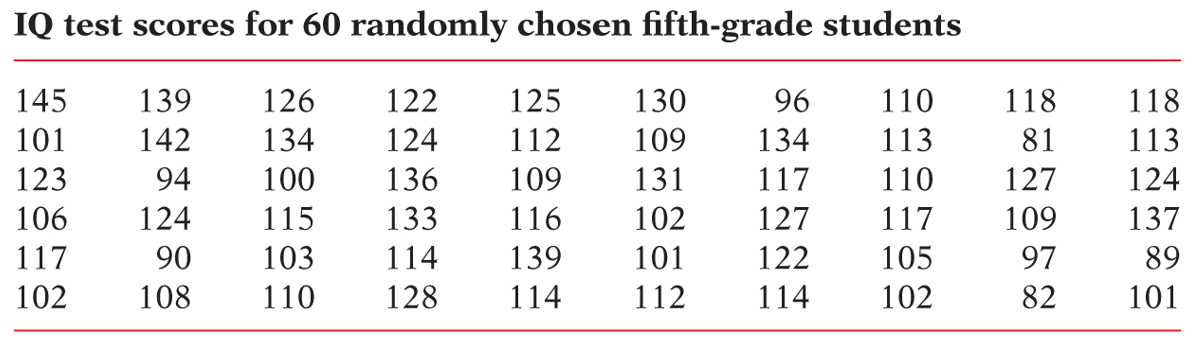
\includegraphics[scale=0.9]{images/iq.png}
\end{center}

We can use a {\bf histogram} to visually inspect the {\em distribution} of these IQ scores.

\begin{center}
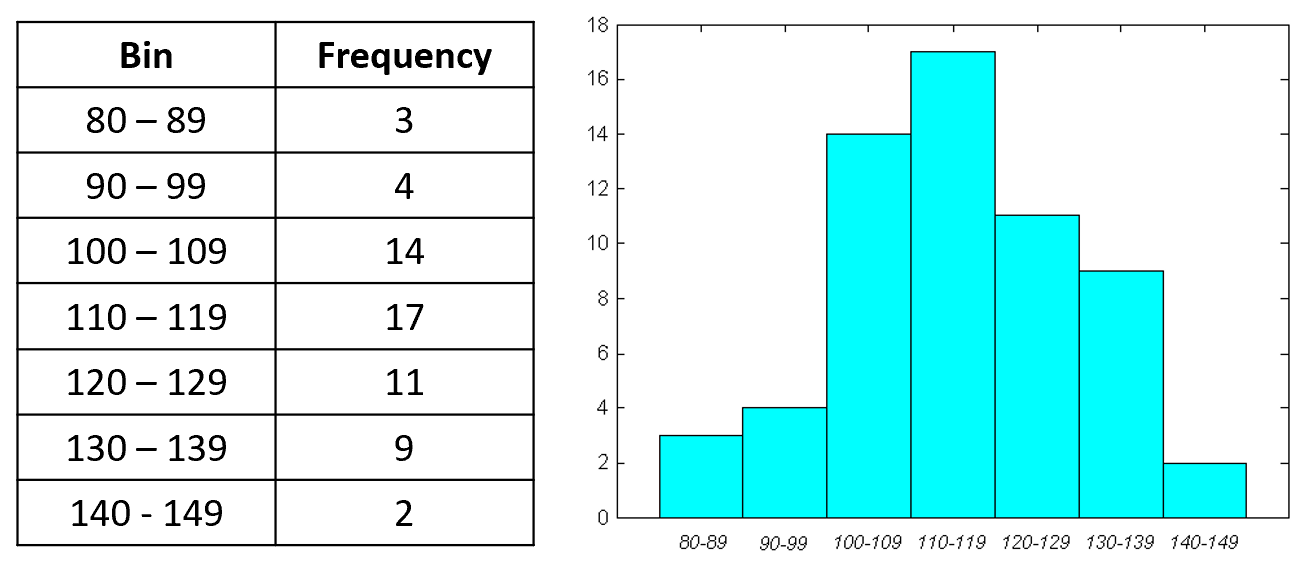
\includegraphics[scale=0.8]{images/hist1.png}
\end{center}

Slightly different choice of bins:

\begin{center}
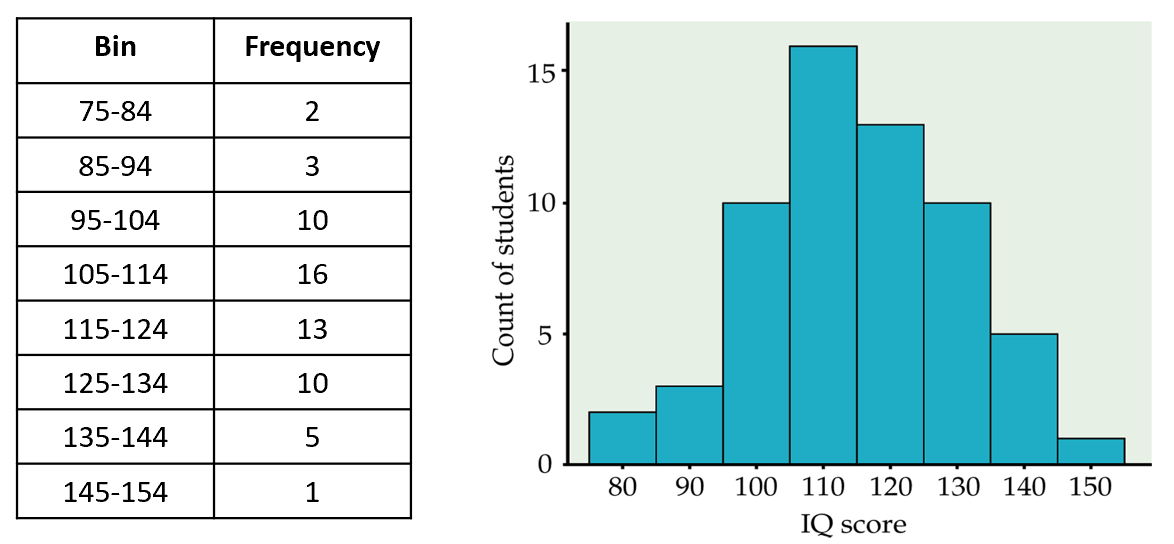
\includegraphics[scale=0.9]{images/hist2.png}
\end{center}

\newpage

Other choices of bins:

\begin{center}
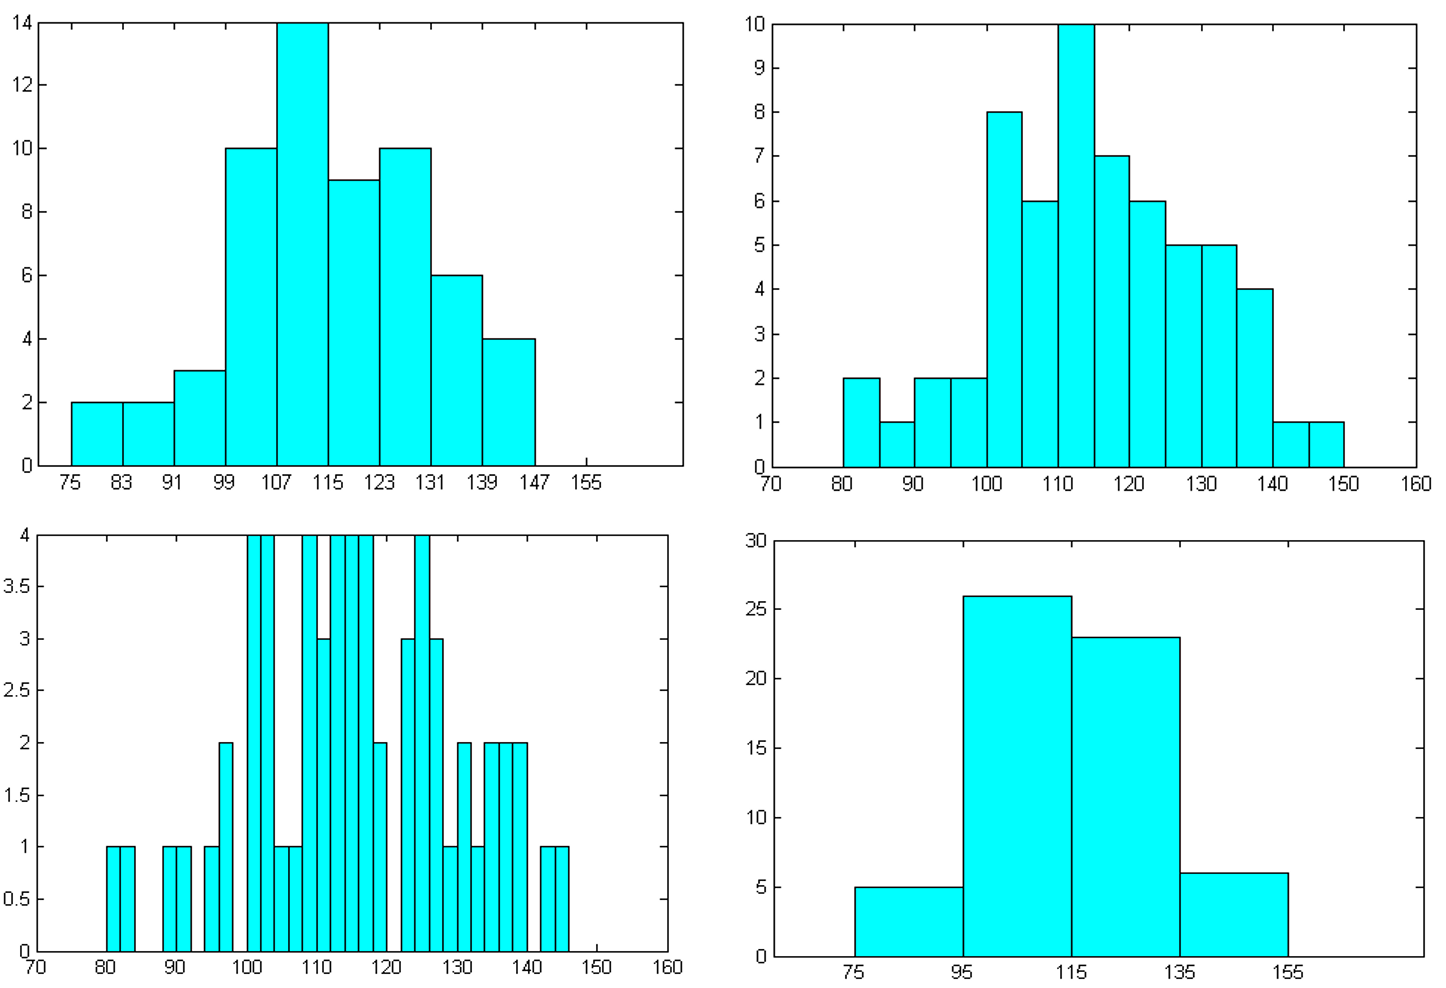
\includegraphics[scale=0.7]{images/hist3.png}
\end{center}

Using relative frequencies instead:

\begin{center}
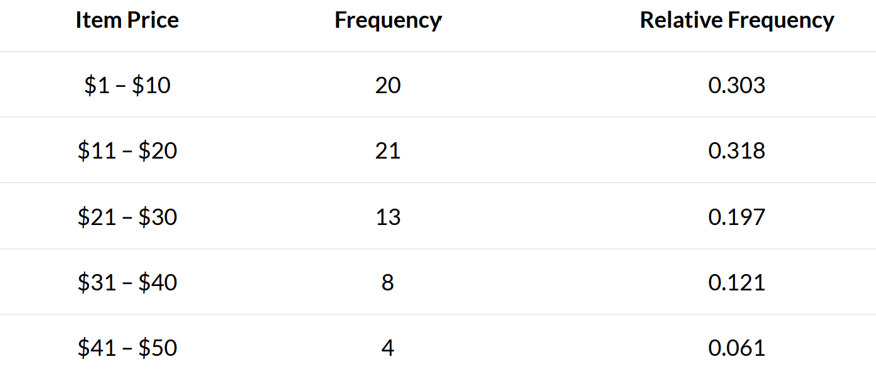
\includegraphics[scale=0.8]{images/prices.png}
\end{center}

\begin{center}
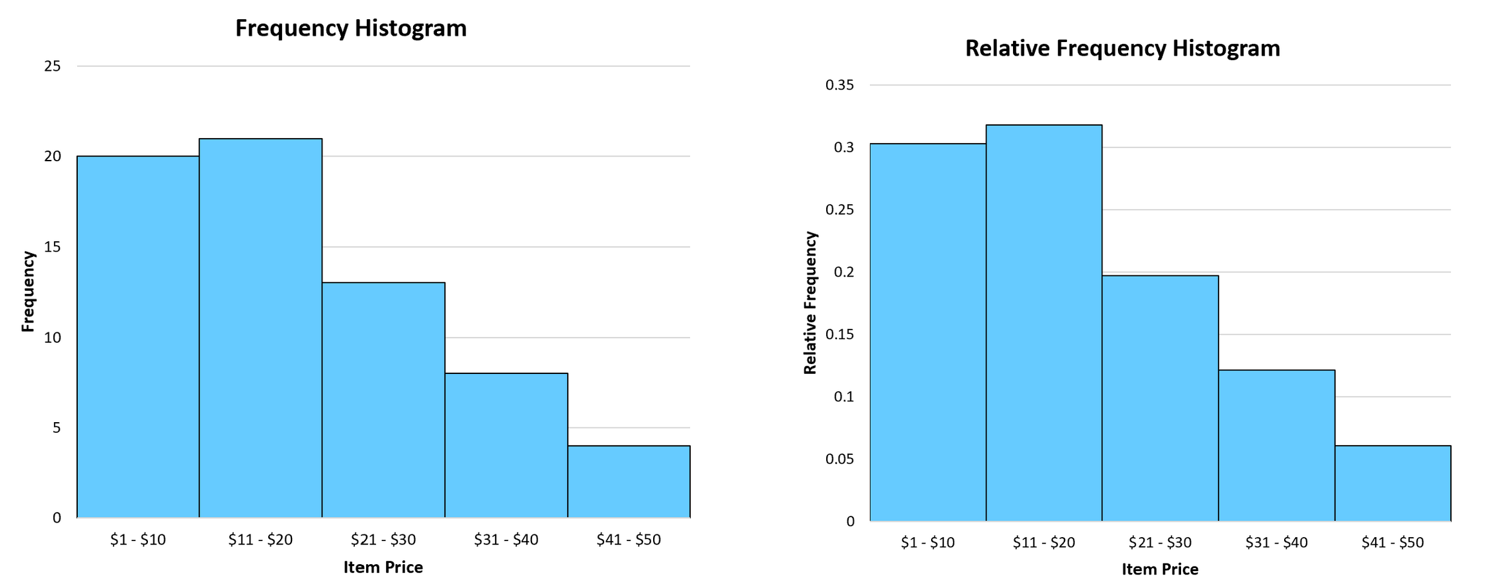
\includegraphics[scale=0.8]{images/hists.png}
\end{center}

\newpage

Using a histogram to identify {\bf outliers}: \vspace{6pt}

\hspace{240pt}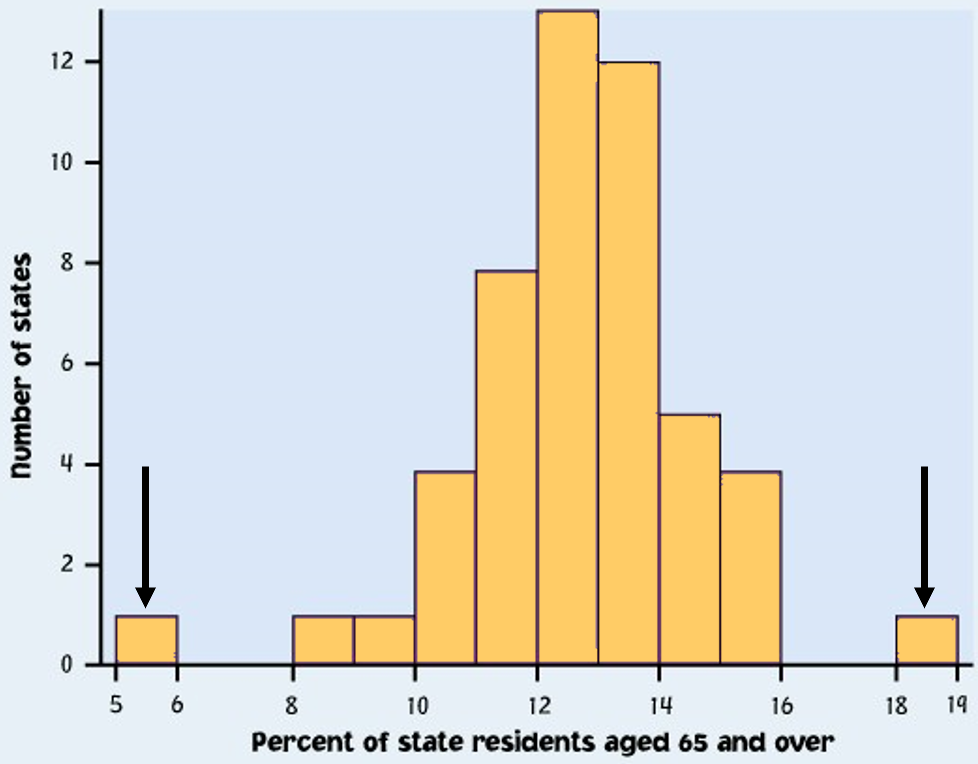
\includegraphics[scale=0.6]{images/hist4.png}

\vspace{20pt}

{\bf Describing Distributions}

\begin{itemize}

\item Shape \vspace{40pt}

\item Center \vspace{40pt}

\item Spread \vspace{40pt}

\item Outliers \vspace{20pt} 

\end{itemize}

\begin{center}
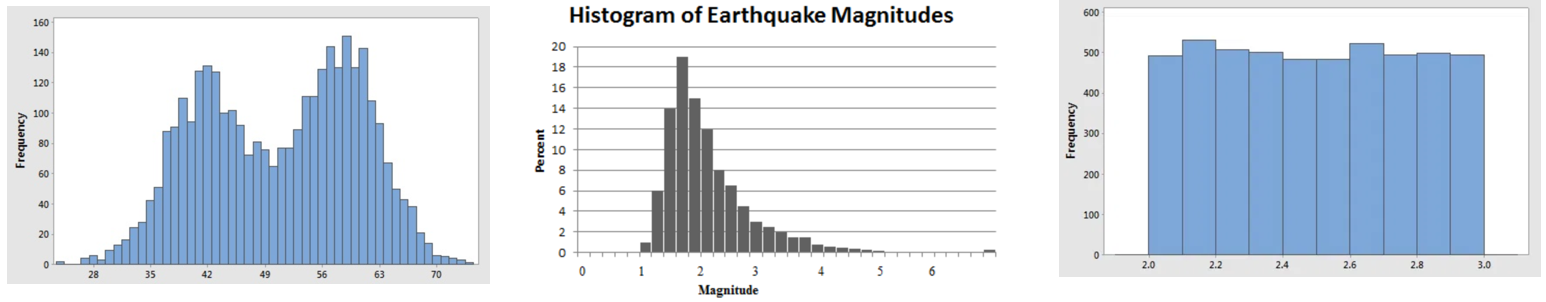
\includegraphics[scale=0.8]{images/hists2.png}
\end{center}

\newpage

Example: A birthday party has 9 attendees of the following ages: 7, 1, 3, 4, 4, 6, 3, 5, 3

\begin{itemize}

\item Notation \vspace{60pt}

\item Measures of center \vspace{240pt}

How does adding a 64-year old to the group change mean and median? \vspace{60pt}

Effect of outliers on mean and median: \vspace{80pt}

\item Median as a percentile

\end{itemize}

\newpage

Same example: Birthday party attendees aged 7, 1, 3, 4, 4, 6, 3, 5, 3

\begin{itemize}

\item Measures of spread: variance and standard deviation \vspace{240pt}

\end{itemize}

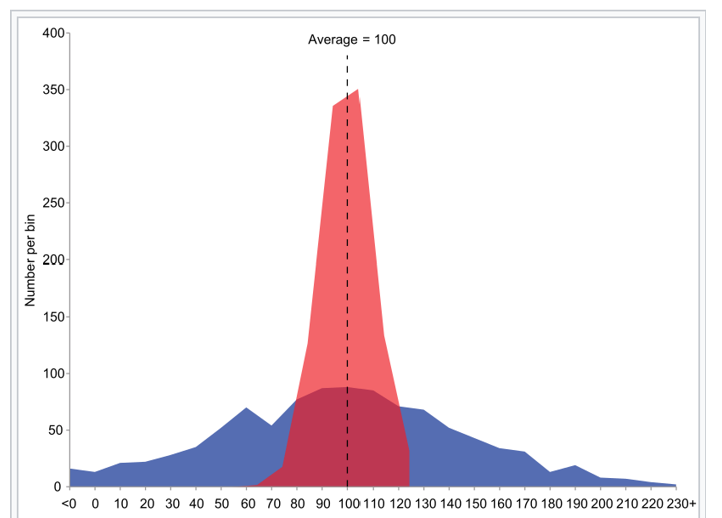
\includegraphics[scale=0.85]{images/sd.png} \hspace{15pt} 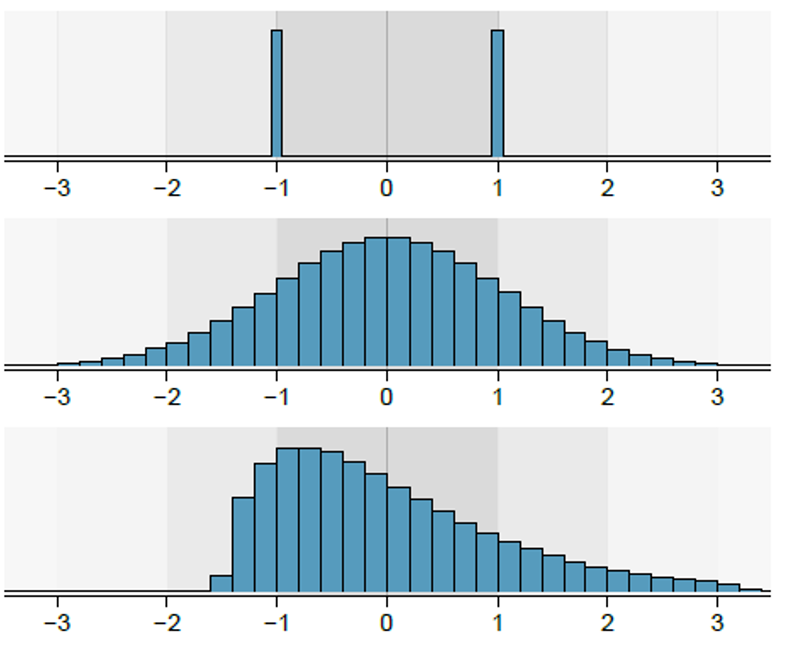
\includegraphics[scale=0.7]{images/sd2.png} \vspace{60pt}

\newpage

Same example: Birthday party attendees aged 7, 1, 3, 4, 4, 6, 3, 5, 3

\begin{itemize}

\item Another measure of spread: IQR \vspace{240pt}

\item IQR criterion for outliers: \vspace{120pt}

\item 5-number summary and box plot:

\end{itemize}

\newpage

Data analysis in Excel: open sheet {\tt unc2017.xlsx}

\label{totalpag}
\end{document}